\begin{wrapfigure}{r}{0.25\textwidth}
\vspace{-4mm}
\centering
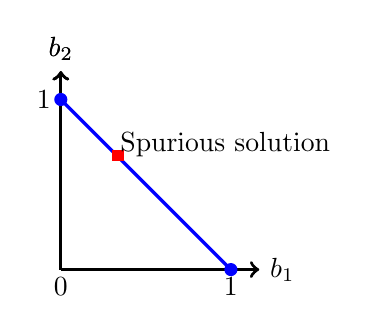
\begin{tikzpicture}[scale=0.72]
\draw[->, very thick] (0, 0) -- (3.5, 0) node[right] {$b_1$};
\draw[->, very thick] (0, 0) -- (0, 3.5) node[above] {$b_2$};
\draw[->, very thick] (0, 0) -- (0, 3.5) node[above] {$b_2$};
\draw[domain=0:3, very thick, variable=\x, blue] plot ({\x}, {3-\x});

%\draw[<-, very thick, dashed] (0.1, 2.6) -- (0.75, 1.95);
%\draw[->, very thick, dashed] (1, 1.8) -- (2.6, 0.2);


\node at (0, -0.3) {0};
\node at (3, -0.3) {1};
\node at (-0.3, 3) {1};
\draw[draw=red, fill=red] (0.92,1.92) rectangle ++(0.18,0.18);
\node at (2.9, 2.2) {Spurious solution};
\filldraw[blue] (0, 3) circle (3pt);
\filldraw[blue] (3, 0) circle (3pt);
\end{tikzpicture}
\caption{Solutions found by convex solver can be spurious.}
\label{fig:onehot}
\vspace{-2mm}
\end{wrapfigure}
